\documentclass[convert={density=300,size=1080x800,outext=.png}]{standalone}
\usepackage{tikz}
\usetikzlibrary{arrows.meta, arrows}
\begin{document}

%.. tikz:: 
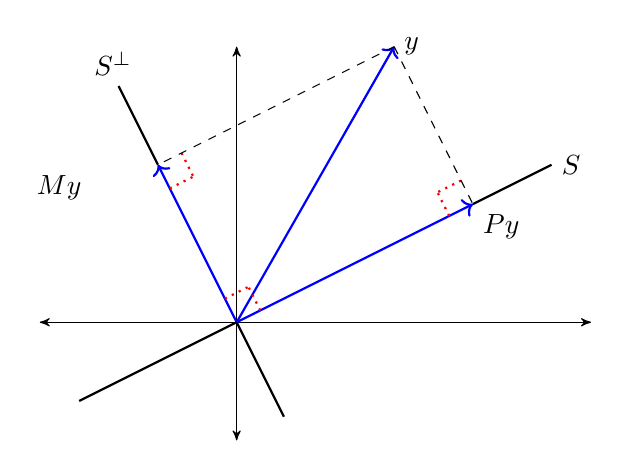
\begin{tikzpicture}
[scale=5, axis/.style={<->, >=stealth'}, important line/.style={thick}, dotted line/.style={dotted, thick,red}, dashed line/.style={dashed, thin}, every node/.style={color=black}] \coordinate(O) at (0,0);
    \coordinate (uhat) at (-0.2,0.4);
    \coordinate (yhat) at (0.6,0.3);
    \coordinate (y) at (0.4,0.7);
    \coordinate (S1) at (-0.4,-0.2);
    \coordinate (S2) at (0.8,0.4);
    \coordinate (S3) at (-0.3,0.6);
    \coordinate (S4) at (0.12,-0.24); 
    \draw[axis] (-0.5,0)  -- (0.9,0) node(xline)[right] {};
    \draw[axis] (0,-0.3) -- (0,0.7) node(yline)[above] {};
    \draw[important line,blue,thick, ->]  (O) -- (yhat) node[anchor = north west, text width=4em] {$P y$};
    \draw[important line,blue, ->]  (O) -- (uhat) node[anchor = north east, text width=4em] {$M y$};
    \draw[important line,thick] (uhat) -- (S3) node [anchor = south east, text width=0.5em] {$S^{\perp}$};
    \draw[important line,thick] (O) -- (S4);
    \draw[important line, thick]  (S1) -- (O) node[right] {};
    \draw[important line, thick]  (yhat) -- (S2) node[right] {$S$};
    \draw[important line, blue,->]  (O) -- (y) node[right] {$y$};
    \draw[dotted line] (-0.03,0.06) -- (0.03,0.09);
    \draw[dotted line] (0.06,0.03) -- (0.03,0.09);
    \draw[dotted line] (0.54,0.27) -- (0.51,0.33);
    \draw[dotted line] (0.57,0.36) -- (0.51,0.33);
    \draw[dotted line] (-0.17,0.34) -- (-0.11,0.37);
    \draw[dotted line] (-0.14,0.43) -- (-0.11,0.37);
    \draw[dashed line, black] (y) -- (yhat);
    \draw[dashed line, black] (y) -- (uhat);
\end{tikzpicture}

\end{document}